\chapter{Background \& Related Work}
\label{ch:background} 

The background and related work in the subject of this project will be introduced in this chapter, from existing CV checkers, and special unstructured resume data, to the NLP and Machine Learning techniques related to resume processing or information extraction. Moreover, some relevant systems will also be mentioned, regarded as the reference or the future work of our project.


\section{Existing CV Checker}

During the decades, e-recruitment in the recruitment process has been augmented, which has caused a significant change in the recruitment environment \cite{barber2006recruitment}. With the rapid development of the e-recruitment system, an increasing number of candidates uploading their resumes online to apply for positions \cite{mittal2020methodology}, and numerous applications are implemented for the recruiters to screen the resumes of candidates. For instance, \cite{amin2019web} proposed a web application that can use NLP and machine learning techniques to compare the resumes and the job profile requirements, then score and rank all the candidate resumes. Furthermore, a Smart Apply Ranker system \cite{mohamed2018smart} is designed for candidates' recommendation of IT companies in a semantic way. In this case, to better match the resume-screened system, CV checkers are developed for job seekers as effective tools in this e-recruitment landscape.


Several CV checkers have being implemented to help people optimize their resumes to get more interviews.  \href{https://careerset.com/}{CareerSet} is a powerful CV review solution aiming on students to improve the quality of their CVs. According to \cite{laffey_2022}, this platform has been a significant tool for dozens of universities' Career Development Centre for their students' career guidance. After the student uploads the resume, CareerSet will return the feedback and the recommendations, which contain four main parts, impact, brevity, style and others, including word-use check, information check, spell check, et cetera. \href{https://www.jobscan.co/}{Jobscan} is another effective CV checker which 
can compare the resume and the target job description, rate the resume and give feedback on skill match, title match and format check.

Those existing CV-checking applications provide helpful platforms for job seekers to view their resumes automatically and modify CVs to fit the target job position better. Because of the business secrete, the inside algorithms of those applications are not open-sourced. In this project, we would focus on researching the NLP techniques and machine learning algorithms to create an AI-powered CV checker which refers to the functions of JobScan and CareerSet.


\section{Resume Data}

Unstructured data refers to data without a pre-defined data model \cite{gharehchopogh2011analysis} and is not coded as the pre-defined analytical categories \cite{boulton2006analysis}. The unstructured data is normally text-heavy, and sometimes contains information such as dates and numbers \cite{enwiki:1077284794}. Resumes are a typical source of unstructured data \cite{van2015difference}, and can be learnt and understood by computers through NLP \cite{hirschberg2015advances}. According to \cite{zhang2018resumevis}, resume data indicates the personal profile and work experiences of the individuals, and RA (Resume Analysis) studies could be applied to many applications such as recruitment prediction. To find out the latent semantic information from the resumes and comprehensively understand of those unstructured data, Zhang and Wang \cite{zhang2018resumevis} proposed a Visual Analytics System based on text mining combined with visualized techniques which have been proved effective by over 2,500 resumes from government officials. 

PDF is a standard format for resumes containing various information of the recruiters \cite{chen2016information}, and Chen, Gao and Tang researched on the information extraction from the resumes in PDF format \cite{chen2016information}. They proposed a hierarchical extraction method, which splits the PDF page into blocks based on heuristic rules and a Conditional Random Field model is used to classify the blocks by applying content-based features and layout-based features from the documents. Our project can refer to this PDF extraction method. The following figure \ref{fig:2} shows the structure of the resume. Based on this hierarchical structure, Kudatarkar et al.\cite{kudatarkar2015survey} came up with an approach including both grammar and probabilistic parameters in the parser to build the concepts in the resumes.

 \begin{figure}[H]
    \centering
    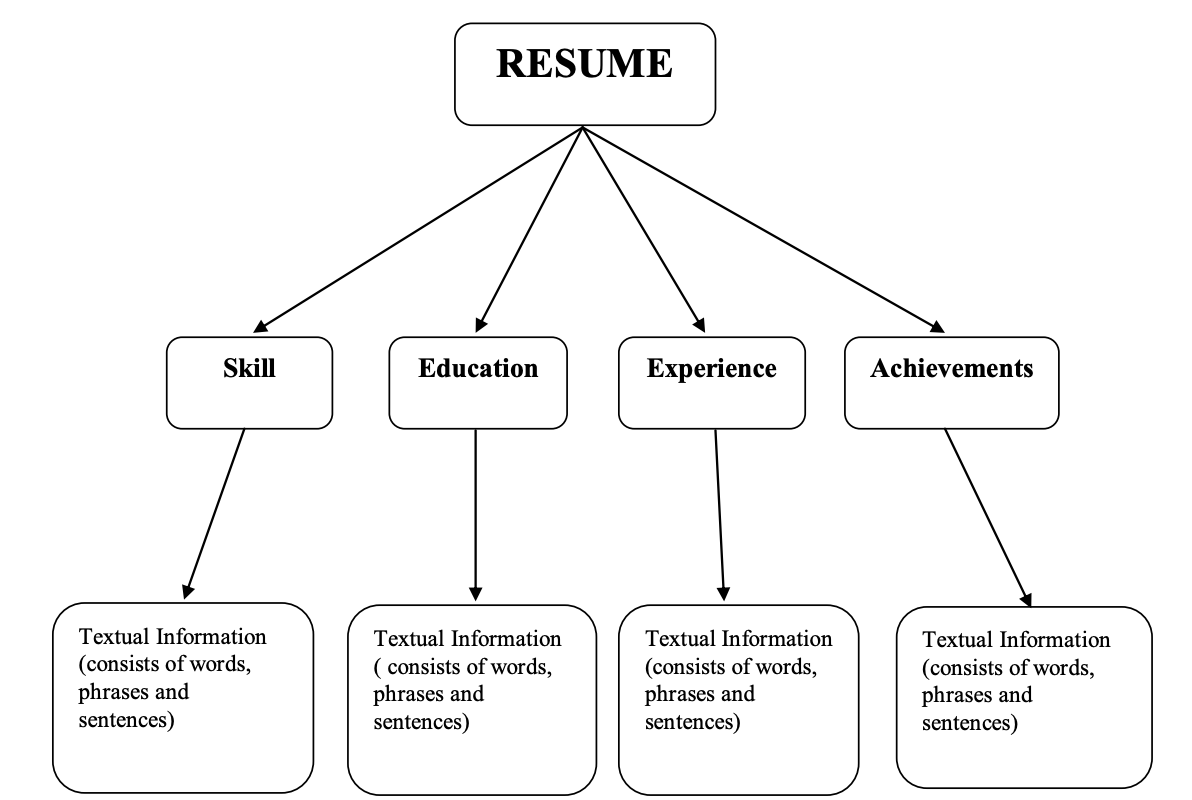
\includegraphics[width=0.9\textwidth]{images/resume_structure.png}
    \caption{Hierarchical Structure of Resume \cite{kudatarkar2015survey}}
    \label{fig:2}
\end{figure}



\section{NLP Techniques}

Natural Language Processing, also known as computational linguistics, is a subarea of computer science which uses computational approaches to learn to comprehend and produce natural language, and has proliferated over the past decades \cite{hirschberg2015advances}. NLP techniques are normally used to handle communication, including lexical, syntax and semantic analysis \cite{alamelu2021resume}. Before this project, there have been many implementations using NLP techniques to process resumes. \cite{alamelu2021resume} created a web application to help the resume screening process more accessible and straightforward. This web application can compare the submitted resumes with the job description and then rank resumes by the matching rate to find the candidates for the job. A modified NER (Named Entity Recognition) model is used to identify the crucial items in resumes, such as skills and work experience, and Cosine Similarity could compute the matching rate. 

Keyword extraction is also a vital process to understand the resumes better. Extracting keywords is complex because natural language is diverse and the concept of keyword is hard to define \cite{firoozeh2020keyword}. Hussey, Williams and Mitchell proposed a study on the comparison of automatic keyphrase extraction method \cite{hussey2012automatic}, which focuses on the extracted performance and result of different features. Moreover, Hasan and Ng researched the errors of the keyphrase extraction system \cite{hasan2014automatic}. As for the extraction features of resumes, the keyword extractors might be different from other systems. Though almost all resumes have unique structures, there can be found a typical hierarchical layered structure for resumes \cite{finn2004multi}, which can make the keyword extraction task for resumes easier. 

Kopparapu and Kumar \cite{kopparapu2010automatic} proposed a system to extract resume information automatically. This system can extract six different necessary informative fields, such as work experience, e-mail address and skill set, from the unstructured resume data by a series of NLP techniques, and can handle resumes in multiple forms. The extraction processes are implemented by part heuristics and part pattern matching techniques, which can be used in our project.
 \begin{figure}[H]
    \centering
    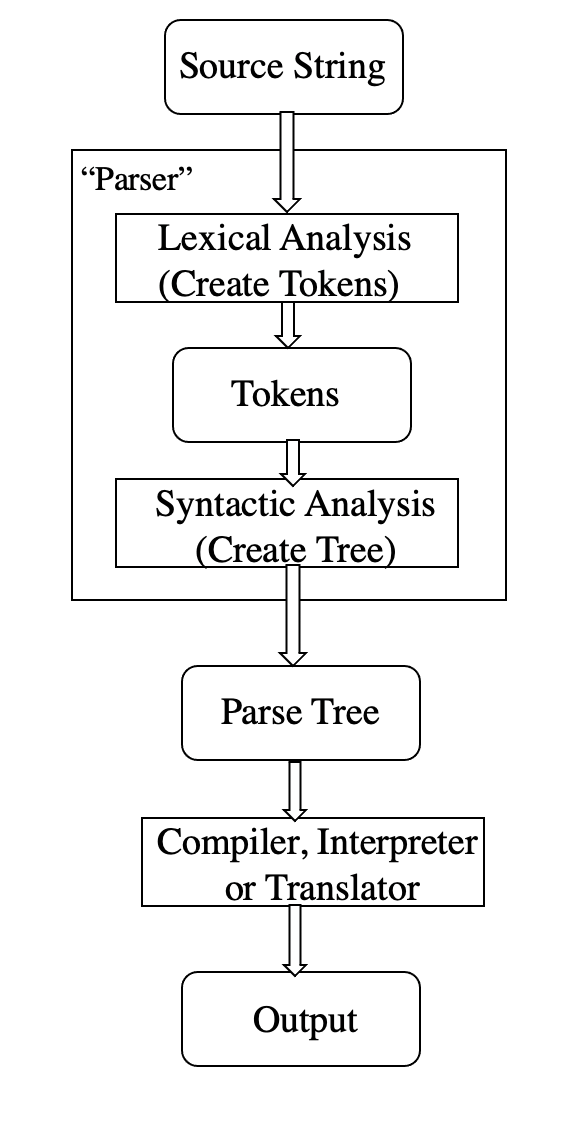
\includegraphics[width=0.35\textwidth]{images/model.png}
    \caption{Model Design \cite{sanyal2017resume}}
    \label{fig:1}
\end{figure}


Sanyal et al. \cite{sanyal2017resume} designed a model to parse all the relevant data in resumes including contact information, education details and work experience, and transform them into JSON format. The parser used Lexical Analysis, Syntactic Analysis and Semantic Analysis these three NLP techniques to constrain the information in the resumes. The Lexical Analysis part tokenized the input resumes data, and then used NER to extract the related information in each segment. The parser generated the parse tree, which can represent and directly reflect the syntax of the input data, through Syntactic Analysis. As for Semantic Analysis, it could study the meaning and the structure of the data, and could find the language-independent meanings. After three analyzers, the system will generate JSON data to represent the resume and store it in the database for further analysis. The model design is shown in the above figure \ref{fig:1}, which would be helpful for our project.



Identifying the features such as skills in the resume is another key point in a CV checker. An ontology-based resume searching system is developed to match CVs and job descriptions \cite{phan2021ontology}. Resume Ontology includes classes, properties and relational concepts, which can represent the resume in a semantic way \cite{ccelik2013towards}. Computer Science Ontology (CSO) Classifier is an unsupervised method that can take the metadata as the input and return the topic category of the document according to CSO \cite{salatino2019cso}. Phan et al. \cite{phan2021ontology} 's system can parse and processes the uploaded CV, extract the skills by CSO Classifier and match the CV to the target position by the calculated similarity of the skill graph. Figure \ref{fig:3} illustrates the process of the architecture of this Resume Searching system, and the design of our project could be referred to it.

 \begin{figure}[H]
    \centering
    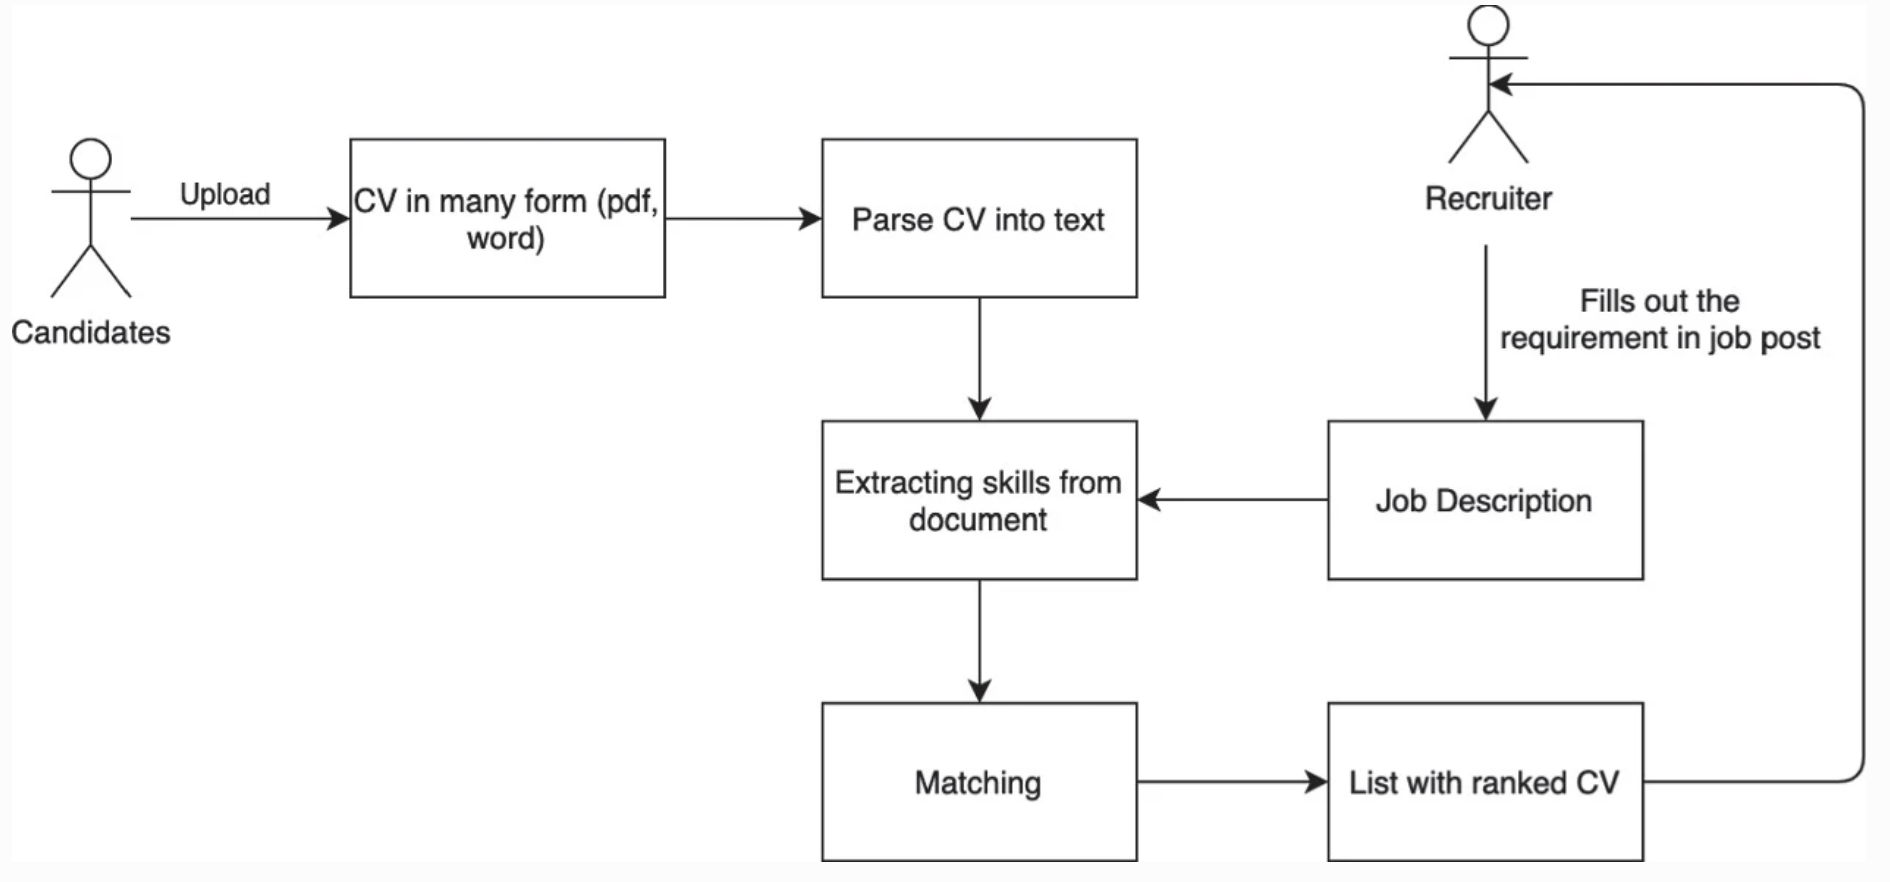
\includegraphics[width=0.9\textwidth]{images/architecture.png}
    \caption{Architecture of the Resume Searching System \cite{phan2021ontology}}
    \label{fig:3}
\end{figure}


In \cite{maheshwari2010approach}, an approach has been proposed for special skill extraction for companies to filter resumes and reduce the number of candidates. It can extract the skill type features and the skill value features, then calculate the specialness value degree of those features to determine and organize the particular skill type. The features could be organized into three levels, common features, common cluster features and special features by setting a similarity threshold value. This proposed framework can help the user or the recruiters to check the resume based on special skill type and get the corresponding skill values. This system is more likely to be used for selecting the suitable resume from a set of similar resumes on the basis of special skills. However, some ideas in it such as skill classification could be considered in our CV checker. 


\section{Machine Learning Techniques}

The machine learning algorithm, regarded as a part of artificial intelligence \cite{enwiki:1103198106}, can build the model based on the sample data to make predictions or decisions without specific program \cite{koza1996automated}. Techniques based on machine learning are widely used in various areas in which it is hard to be implemented by the traditional algorithm for the tasks such as medicine and speech recognition \cite{hu2020voronoi}. Nowadays, machine learning approaches are ubiquitous in NLP tasks, and have been proved to perform well on tasks such as Part of Speech tagging, Named Entity Recognition and Sentiment Analysis \cite{socher2012deep}. According to \cite{sinha2021resume}, it is a difficult task to extract information from human language since human language is diverse and ambiguous, and it can be expressed in many different ways. Machine learning models play an important role in reducing ambiguity and capturing linguistic information from the human language \cite{jurafsky2000speech}. Before using ML techniques, NLP tasks are implemented by rule-based approaches and should be coded manually \cite{khan2016survey}. Khan et al. \cite{khan2016survey} reported a comprehensive survey in machine learning and NLP domain to discuss different existing ML models applied in computational linguistics for disambiguation. 

Machine learning algorithms can also be used to analyze unstructured resume data. Sinha et al. \cite{sinha2021resume} discussed and evaluated several machine learning techniques for resume parsers. Those CV parsers analyze the context of the document by semantic search to obtain reliable and comprehensive results \cite{sinha2021resume}. Sentence segmentation is a vital task in order to extract definite information from the CVs. The rule-based approach uses a set of punctuations such as '.',';','?' to detect the boundary of the sentence \cite{reynar1997maximum}, but when encountering special situations such as abbreviations, it will be failed \cite{kiss2006unsupervised}. Under these circumstances, supervised machine learning methods such as decision tree could be used to classify the punctuations and decide the sentence boundaries more accurate \cite{riley1989some}. Generally, supervised learning needs to be provided input and output by human, and involves a large set of labelled training data to obtain a good performance \cite{saravanan2018state}. An unsupervised approach was proposed by Kiss and Strunk \cite{kiss2006unsupervised}, which used type-based classification for sentence segmentation by analyzing and annotating the word in the full text. Additionally, besides segmenting the sentences, statistical approaches could also be used in the tokenization task. The statistical approach used scanning hidden Markov model (HMM) boundary detector modules to tokenize \cite{jurish2013word}. Above is the usability of machine learning methods in the textual data processing. 

In e-recruitment, machine learning techniques are widely used to screen, classify and rank applicants automatically. Tejaswini et al. \cite{tejaswini2021design} used K-nearest Neighbours (KNN) algorithm to calculate the distance between resumes and the target job description and return the top K resume choices. \cite{vamsi2021resume} used Naive-bayes and one-vs-rest classifier to process and segregate resumes on the basis of knowledge and technical expertise. Ali et al. \cite{ali2022resume} evaluated nine ML models on Resume Classification System (RCS), and the Support Vector Machine (SVM) classifier got the best performance with over 96\% accuracy on the resume dataset. The results indicated that NLP and machine learning techniques could be used to develop the efficient RCS \cite{ali2022resume}. In our project, ranking or classifying resumes would not be involved, but the idea that combining NLP with machine learning approaches in resume-related projects could be taken into consideration.

Deep learning is a subfield of machine learning which aims to develop high-level features and representations from the complex explication input by multiple layers \cite{deng2014foundations}. \cite{gunaseelan2020automatic} proposed a system that can extract information such as skills, education and experience from the resume by a multi-level classification approach. Ontology matching technique can be used to recognize the technical skills by part of speech patterns, but it relies extremely on the completeness of the database \cite{chifu2017system}. In this situation, with the development of computational ability, deep learning models such as LSTM are used for Named Entity Recognition for segment information extraction \cite{gunaseelan2020automatic}. \cite{chen2018two} implemented a text block classification method by regarding the text as blocks based on the title words of the resume documents. But since the unstructured characteristic of resumes, it is complicated to define this kind of document as separate blocks. Ayishathahira et al. \cite{ayishathahira2018combination} used Convolutional Neural Network (CNN) segmentation model to segment the information into educational, occupational and others, and CRF and BiLSTM are developed for information extraction. \cite{kumar2019supervised} came up with a supervised deep learning algorithm regarding the skills as relevant keywords to extract skills from the resume by predicting the relevant keywords. The importance of each word in the data are calculated to indicate the probability of a word being the skill.

Many other machine learning algorithms other than deep learning approaches could be used for the above skill extraction task. \cite{jo2017using} used K-Nearest Neighbors for text segmentation, which calculates the similarity among the feature vectors and classifies the sentences into specific groups based on the similarity. Ensemble learning combines multiple learning algorithms together to obtain better performance than a single learner \cite{enwiki:1100411098}. \cite{goudjil2018novel} proposed a multi-class SVM approach to learn the knowledge of the data by selecting the most informative samples. 

In addition, identifying the skills in the job description to check the resume is regarded as a significant task in the CV checker as well. Liu et al. \cite{liu2021learning} proposed a Multi-Graph Neural Network based Skill Prediction (MGNSP) model to define the job skill requirements for the positions. They built three networks for job, skill and job-skill to get the recommended skills for a job position. Job network can aggregate the information from the neighbors of every job description to handle the false predictions, Skill network models the skills' correspondence and Job-Skill network combines the job descriptions and skills together to get the suggested skills from the similar descriptions of the position. The prediction of skills would not be used in this project, but the three networks to get the aggregation and correlation could help to understand the job description data. Like the unstructured resume data, deep learning models such as LSTM and biLSTM are able to recognize the skills expression from the job posts based on time series data \cite{baad2019automatic}. Moreover, Zhou et al. \cite{zhou2016quantifying} adapted a systematic method to measure the relevance of the skills to the job titles depending on the job description and skill keyword representation. In their research, the skill relevance is assessed by TF-IDF (Term Frequency - Inverse Document Frequency) based score and the dispersion of the skill expression over the positions. The above approaches, such as skill ranking and skill relevance across the job description could be considered as the future work for our project.